\section{The E and B statements, reconsidered}
\label{sec:eb}

The draft makes three claims about the polarization structure of the FK
term. They deserve separate treatment, because one is exactly right, one is
right only in a limit, and one is a theorem rather than a measurement.

\subsection{Which channel carries E minus B}

The claim is stated in \code{conclusion.tex}: the FK contribution to
$\xi_+$, which is $C_\ell^{EE}+C_\ell^{BB}$, is sourced by
$\langle\Phi_{00}\Psi_+\Psi_+\rangle+\langle\Phi_{00}\Psi_\times\Psi_\times\rangle$,
its counterpart in $\xi_-$, which is $C_\ell^{EE}-C_\ell^{BB}$, by the
difference, and the difference ``vanishes for a statistically isotropic
driving field''.

Which vertex channel that is can be read straight off the callable's
real-basis reconstruction rather than derived. The coupling tensor is
filled as
\[
  K_{011}=\tfrac12(\zeta_{TPP}+\zeta_{Bmod}), \quad
  K_{022}=\tfrac12(\zeta_{Bmod}-\zeta_{TPP}), \quad
  K_{111}=\tfrac14(\zeta_{PPP}+3\zeta_{Dmod}), \quad
  K_{122}=\tfrac14(\zeta_{Dmod}-\zeta_{PPP}),
\]
so that, verified to machine zero,
\[
  K_{011}+K_{022}=\zeta_{Bmod}, \qquad K_{011}-K_{022}=\zeta_{TPP},
\]
\[
  K_{111}+K_{122}=\zeta_{Dmod}, \qquad
  K_{111}-K_{122}=\tfrac12(\zeta_{PPP}+\zeta_{Dmod}).
\]
The sums feed $\xi_+$ and the differences feed $\xi_-$. In real components
$\zeta_{Bmod}=\langle\Phi_{00}(\Psi_+^2+\Psi_\times^2)\rangle$ and
$\zeta_{TPP}=\langle\Phi_{00}(\Psi_+^2-\Psi_\times^2)\rangle$, so the
draft's claim is exactly the statement $\zeta_{TPP}=0$. Numerically
$\zeta_{TPP}$ dominates the difference: at $\gamma=53'$ on the source shell
it is six times $\tfrac12(\zeta_{PPP}+\zeta_{Dmod})$.

\subsection{The claim is a zero-separation identity}

The isotropy argument is correct where it applies. When all three legs sit
at the same point there is no separation vector, nothing distinguishes
$\Psi_+$ from $\Psi_\times$, and the difference vanishes identically. The
table confirms it: $\zeta_{TPP}$ is exactly zero at $\gamma=0$.

At finite separation the offset leg supplies an axis, $\Psi_+$ and
$\Psi_\times$ are defined relative to it, and there is no reason for the
difference to vanish. Measuring it (Figure~\ref{fig:eb}) gives a clean
answer:

\begin{itemize}
\item $|\zeta_{TPP}/\zeta_{Bmod}|$ rises from zero as $\gamma^4$. The
measured logarithmic slope is $4.00$ at $\gamma<2'$, drifting to $4.2$ by
$5'$ and steepening further above $10'$. The draft's own statement that
$\xi_-$ is ``suppressed as $\gamma^4$'' is therefore exactly right as a
small-angle scaling. \emph{Superseded at the converged cutoff}: the slope
is $3.94$ at $0.5'$ but $2.51$ by $1.3'$ and below unity above $2'$, so the
$\gamma^4$ law survives only below an arcminute (Section~\ref{sec:cutoff}).
\item That suppression is relative to a channel which is itself falling, so
the ratio grows quickly. It passes $1\%$ at $\gamma=9.0'$, $10\%$ at
$13.6'$, $50\%$ at $18.3'$, and $1$ at $\gamma=21.9'$.
\end{itemize}

So the correct statement is not that the difference vanishes but that it is
$\gamma^4$-suppressed, and $\gamma^4$-suppressed only means small below
about ten arcminutes. Beyond about twenty arcminutes the difference channel
is as large as the sum channel. Both scales sit inside the range the draft
plots and inside the range cosmic-shear surveys measure.

\begin{figure}[t]
\centering
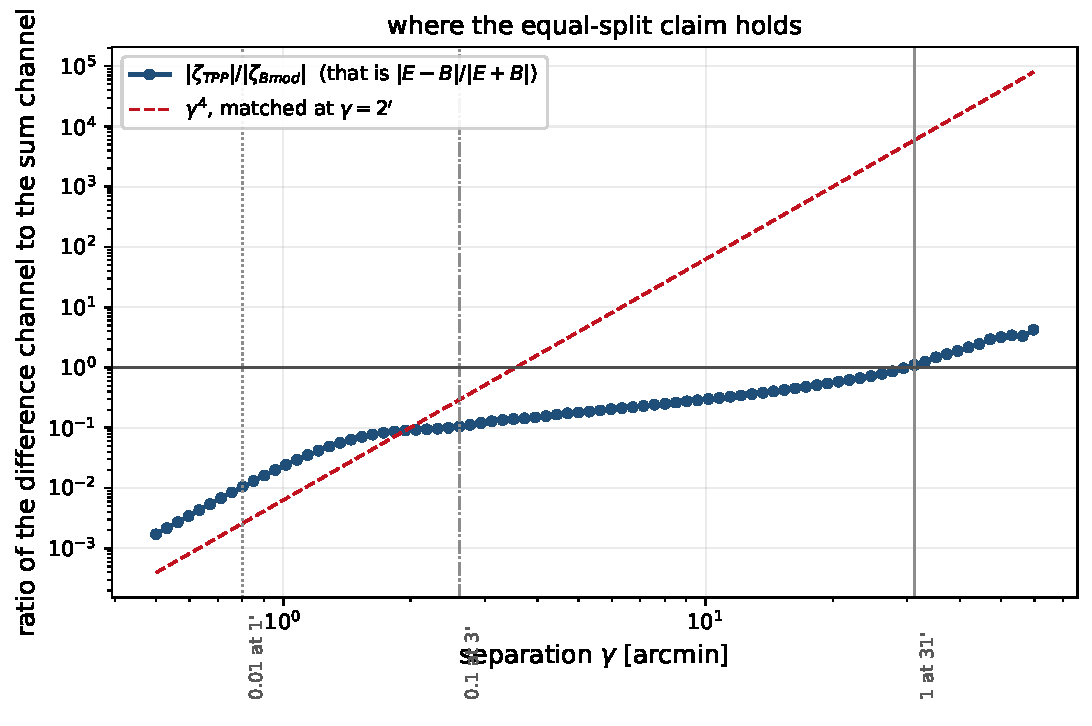
\includegraphics[width=0.78\textwidth]{figures/eb_structure.pdf}
\caption{The ratio of the difference channel $\zeta_{TPP}$, which carries
$C_\ell^{EE}-C_\ell^{BB}$, to the sum channel $\zeta_{Bmod}$, which carries
$C_\ell^{EE}+C_\ell^{BB}$, on the source shell. The dashed line is a
$\gamma^4$ reference matched at $2'$. Beyond about $60'$ the sum channel
passes through zero and the ratio stops being meaningful, so the plot
stops there. Produced by \code{code/rebuild/fig\_eb\_structure.py}.}
\label{fig:eb}
\end{figure}

\subsection{What the corrected calculation gives}

With the vertex resolved, $\xi_-$ is no longer at the numerical floor and
the two polarizations no longer carry equal power. In the corrected run,
after the callable corrections of Section~\ref{sec:callablefix},
$\max|\Delta C_\ell^{EE}|=1.69\times10^{-6}$ and
$\max|\Delta C_\ell^{BB}|=7.03\times10^{-7}$, so $B/E\simeq0.42$ in power
rather than $1$. \emph{Superseded}: a ratio of two maxima is not a stable
number, because the two maxima sit at different multipoles and both sit in
the low-$\ell$ region that Section~\ref{sec:afterwards} shows is not
converged. Taken over $\ell\ge2$ it reads $1.57$, over $\ell\ge20$ it
reads $0.54$. The stable statement is per multipole, over the converged
band: $\Delta C_\ell^{BB}/\Delta C_\ell^{EE}$ falls from $0.95$ at
$\ell=60$ to $0.42$ at $\ell=1500$, median $0.63$. Against the Order-0 $E$-mode band power that is a B-mode
contribution of a few tenths of a percent.

The permutation caveat that an earlier version of this number carried is
gone: $\xi_-$ is carried by the spin channels, which were the ones the
symmetrised tensor fill mishandled, and correcting it moves $B/E$ from
$0.36$ to $0.42$. What remains is the cutoff of Section~\ref{sec:cutoff},
which raises the whole FK term; the ratio is more robust than the
amplitude.

That a B-mode exists at all is not surprising at this order, and it is the
part worth keeping: an Order-2 term sourced by driving-field
non-Gaussianity generates shear B-modes, and B-modes are the standard null
test in cosmic shear. A prediction at the few tenths of a percent level is
small, but it is a prediction, and the draft currently states a different
one.

\subsection{The parity null is a theorem, not a measurement}

$C_\ell^{EB}$ is exactly zero in the corrected run, as in the deployed one.
This survives, and the reason should be stated plainly. Under a reflection
about the separation axis $\Phi_{00}\to\Phi_{00}$, $\Psi_+\to\Psi_+$ and
$\Psi_\times\to-\Psi_\times$, so $\langle\Phi_{00}\Psi_+\Psi_\times\rangle$
equals minus itself and vanishes. The implementation encodes this
structurally: every coupling-tensor entry with an odd number of index-2
slots is never assigned and stays zero, and the tabulated channels carry
only the real parts that populate the even entries.

The consequence is that the parity panel of the draft's
$C_\ell^{EB}$ figure is not an independent numerical test of parity in the
driving field. The input has $C_\ell^{EB}=0$ by construction. What the
figure does demonstrate, usefully, is that the curved-sky transform and the
fold do not leak $E$ or $B$ power into $EB$ at any level above the
numerical floor. That is worth saying, and it is a different statement from
the one a reader would infer.

\subsection{Recommended wording}

\begin{itemize}
\item Keep: the $\gamma^4$ suppression of $\xi_-$, which is measured to
hold with slope $4.00$ at small separation.
\item Keep: $C_\ell^{EB}=0$, stated as a parity theorem and as a check on
the transform rather than as a measurement of the driving field.
\item Replace: ``the FK power splits equally between the two
polarizations, $\Delta C_\ell^{EE}=\Delta C_\ell^{BB}$'' by a statement
that the split is equal in the coincident limit and that away from it the
two polarizations separate, the B-mode falling from $0.95$ of the E-mode
power at $\ell=60$ to $0.42$ at $\ell=1500$. The ``reaches the size of the
sum near $20$ arcminutes'' form of this item was measured at the deployed
cutoff and does not survive: at the converged cutoff $\xi_-/\xi_+$ is
$0.21$ at $22'$ and does not approach unity until about a degree.
\item Replace: ``FK cancels below the plotted floor'' in $\xi_-$ and
$\xi_{\kappa\gamma_t}$ by the corrected magnitudes, with the permutation
caveat attached.
\end{itemize}
